\section{Translating RTL to Software Netlists}\label{sec:v2c}

The main challenges in translating Verilog faithfully into C are presented by its hardware-oriented elements. Many Verilog statements have no direct analogue in C.  Examples include
initial blocks, always blocks, generate statements, and procedural assignments
(blocking and non-blocking). Verilog also has special hardware-oriented operators, such as part-select, bit-select from vectors, concatenation, and reduction. Finally, Verilog supports the 4-valued data types
reg, wire, and integer.  And all these constructs are combined with
parallelism.

In view of this complexity, our translation is deliberately direct and transparent: we aim to
preserve the RTL's structure and refrain from optimization and abstraction. Fidelity of the
resulting C to the semantics of the Verilog is prioritised, and we rely on
downstream software analysis tools for efficiency.

Our translation is implemented in a tool called V2C~\cite{mtk2016}. The front-end performs Verilog parsing, macro preprocessing, and type-checking. The result is a type-annotated parse-tree, which is then translated into C. There are two main aspects to the translation. The first deals largely with the representation in C of Verilog data values---for example Verilog data types, wires and registers, and Verilog expressions with bit-manipulating operations. This is explained in Sec.~\ref{sec:data}. The second aspect is the scheduling of non-blocking and blocking assignments in Verlog code into a suitable C sequentialization, depending on the their syntactic context. Inter-modular dependencies between the always clocked blocks and the continuous assignment statements are resolved by a dependency analysis. The detail of this part are explained in Section~\ref{sec:dep}.

Translation is followed by code-generation, in which the intermediate expressions and translated module items are converted to ANSI-C program syntax.

\subsection{Verilog Data, Circuit Structures, and Expressions}\label{sec:data}

\subsubsection{Data Model} The data model in Verilog is significantly 
different from C.  Each bit of a C integer value can have 
only two states, namely 0 and 1.  The Verilog HDL
value sets consists of four states, namely 0, 1, $X$ and $Z$.  A value of 0
represents low voltage and value of 1 represents high voltage.  Further,
data values $X$ and $Z$ represent an unknown logic state and a 
high impedance value, respectively.  The simplest synthesis semantics 
for $X$ is treating it as a don't-care assignment, which allows the 
synthesis to choose a 0 or 1 to further improve logic minimization.
V2C treat $X$ and $Z$ states to be non-deterministic as there is no
corresponding C state. 

\Omit{
\subsubsection{Variable declaration} Variables of specific 
bit-width (register, wire) in Verilog is translated 
to the next largest native data-types in C such as 
char, short int, long, long long etc. The default 
variable declaration in C is \texttt{unsigned} except for 
the integer declaration in Verilog which is signed.
}

\subsubsection{Registers, wires, parameters and constants} Verilog supports structural 
data types called \emph{nets}, which are \emph{wire}
and \emph{reg}. The value of wire variables changes 
continuously as the input value changes.  Whereas, 
the \emph{reg} types hold their values until another value is 
assigned to them.  A structure containing all state holding
elements of a module is declared in C to store the register
variables. Wires are declared as local variables in C.  
Verilog Parameters are constants which 
are typically used to specify the width of variables,
for eg., \texttt{parameter identifier = constant\_expression;}.
Parameters are declared as constants in C.  
Verilog also allows the definition of the global constants 
using \texttt{`define} construct, for eg., \texttt{`define STATE 2'b00;},
which is same as the \#define preprocessor directives in C.

\subsubsection{Handling Bit-manipulating operations}
V2C automatically handles complex bit-manipulating operators in Verilog, 
like bit-select or part-select operators from a vector,
concatenation operators, reduction OR, and translates them to the 
semantically equivalent expression in ANSI-C. V2C retains 
the word-level structure of the Verilog RTL and generate 
vectored expressions. Figure~\ref{figure:bit} shows 
Verilog code (at the top) and the generated C expressions 
(at the bottom) which are combinations of bitwise and 
arithmetic operators like bitwise OR, AND, multiplication, 
subtraction, shifts and other C operators.     

%
\begin{figure*}[htbp]
\scriptsize
\centering
\begin{tabular}{l|l|l}
\hline
Bit-select & Part-select (System Verilog) & Concatenation \\
\hline
\begin{lstlisting}[mathescape=true,language=Verilog]
wire [7:0] in1,in2;
reg [7:0] out1,out2;
out1[7:5] = in1[4:2];
out2[6] = in2[4];
\end{lstlisting}
&
\begin{lstlisting}[mathescape=true,language=Verilog]
reg [31:0] in, out;
for(i=0;i<=3;i++) begin
out[8*i +: 8]=in[8*i +: 8];
end
\end{lstlisting}
&
\begin{lstlisting}[mathescape=true,language=Verilog]
wire [7:0] in1, in2;
reg [9:0] out;
out = {in2[5:2],in1[6:1]};
\end{lstlisting}
\\
\hline
\begin{lstlisting}[mathescape=true,language=C]
unsigned char in1,in2;
struct smain { 
 unsigned char out1,out2;
} sm;
sm.out1 = sm.out1 & 0x1f | 
(((in1 & 0x1c)>>2)<<5);
sm.out2 = (sm.out2 & 0xbf)| 
(((in2 & 0x10)>>4)<<6); 
\end{lstlisting}
&
\begin{lstlisting}[mathescape=true,language=C]
struct smain {
 unsigned int in,out;
} sm;
for(i=0;i<=3;i++) {
 x=8*i+(8-1); y=8*i;
 sm.out=(sm.out&!(2^31-2^y))
 |(sm.in&(2^31-2^y)); 
}
\end{lstlisting}
&
\begin{lstlisting}[mathescape=true,language=C]
unsigned char in1,in2;
struct smain { 
 unsigned char out; 
} sm;
sm.out = (((in2 >> 2)
 & 0xF) << 6)|
 ((in1 >> 1) & 0x3F);
\end{lstlisting}
\\
\hline
\end{tabular}
\caption{Handling Bit-select, part-select from vectors and concatenation}
\label{figure:bit}
\end{figure*}
%

\subsubsection{Module Hierarchy with Input/Output Port}
The communication between modules takes place through 
ports, which are signals listed in the parameter list at the 
top of the module. Ports can be of type in, out, and inout. 
Figure~\ref{figure:module-hierarchy} shows an example of 
Verilog module hierarchy on the left and the translated 
code block in C on the right. The output ports are passed 
as reference to reflect the changes in the parent module.
The generated C code preserves the module hierarchy of 
the RTL and produce structurally identical code which 
often helps in mapping C-RTL operations for easier debugging. 

\begin{figure}[htbp]
\scriptsize
\centering
\begin{tabular}{l|l}
\hline
Module Hierarchy &  Code block in C \\
\hline
\begin{lstlisting}[mathescape=true,language=Verilog]
module top(in1, in2);
input [3:0] in1, in2;
wire [3:0] o1, o2;
and A1 (in1, in2, o1, o2);
and A2 (.c(o1),.d(o2),
        .a(o1),.b(in2));
endmodule
// Module Definition              
module and1(a, b, c, d);
input [3:0] a, b;
output [3:0] c, d;
reg [3:0] c;
always @(*) begin
 c = a & b;
end
assign d = 1;
endmodule
\end{lstlisting}
&
\begin{lstlisting}[mathescape=true,language=C]
struct state_elements_and {
 unsigned char c; } sand;
void and(unsigned char a, 
unsigned char b, unsigned 
char *c, unsigned char *d) {
 *d = 1; sand.c = a & b;
}
void top(unsigned char in1, 
        unsigned char in2) {
 unsigned char o1,o2;
 and(in1, in2, &o1, &o2);
 and(o1, in2, &o1, &o2);
}
void main() {
 unsigned char in1,in2;
 top(in1, in2);
}    
\end{lstlisting}
\\
\hline
\end{tabular}
\caption{Handling Module hierarchy with I/O ports}
\label{figure:module-hierarchy}
\end{figure}

\subsection{Assignments and Dependency Analysis}~\label{sec:dep}

\subsubsection{Procedural Assignments}
%
Procedural assignments are used within Verilog 
procedures like always and initial blocks and are of 
two types: \emph{blocking} and \emph{non-blocking}.  
Blocking statements are executed in sequential order. However, blocking
assignments which are triggered from the same event execute
in parallel.  We model the parallelism using an auxiliary variable
for all the blocking assignments that are sensitive to the same event. 
On the other hand, the non-blocking statements always 
execute in parallel for the same clock. To model 
parallelism for non-blocking statements, we 
use shadow-variable based update technique. 
The value of register variables are stored in 
auxiliary variables in the beginning of the clock cycle.  
Each read access to the register variables is then replaced 
by these auxiliary variables. This ensures that 
an assignment to the register variable do not influence the 
subsequent assignments. Figure~\ref{figure:block} shows 
the translation of procedural assignments (shown in top) to 
the equivalent C semantics (shown in bottom).     

\begin{figure*}[htbp]
\scriptsize
\centering
\begin{tabular}{l|l|l}
\hline
Non-blocking assignment & Blocking assignment & Continuous assignment \\
\hline
\begin{lstlisting}[mathescape=true,language=Verilog]
reg [7:0] x,y,z;
wire in = 1'b1;
always @(posedge clk) begin
 x <= in;
 y <= x;
 z <= y;
end
\end{lstlisting}
&
\begin{lstlisting}[mathescape=true,language=Verilog]
reg [7:0] x,y,z;
wire in = 1'b1;
always @(posedge clk) begin
 x = in;
 y = x;
 z = y;
end
\end{lstlisting}
&
\begin{lstlisting}[mathescape=true,language=Verilog]
wire in;
reg a,b,t;
wire a = in;
wire c = b; wire d = c; 
always @(posedge clk) begin
 b <= a;
 t <= b;
end 
\end{lstlisting}
\\
\hline 
\begin{lstlisting}[mathescape=true,language=C]
struct smain { 
unsigned char x,y,z; } sm;
unsigned char xs,ys,zs;
 _Bool in = 1;
// save register variables
 xs=sm.x;ys=sm.y;zs=sm.z;
// update register variables
 sm.x = in;
 sm.y = xs;
 sm.z = ys;
\end{lstlisting}
&
\begin{lstlisting}[mathescape=true,language=C]
struct smain {
unsigned char x,y,z;}sm;
 _Bool in = 1;
// clocked block
 sm.x = in;
 sm.y = sm.x;
 sm.z = sm.y;
\end{lstlisting}
&
\begin{lstlisting}[mathescape=true,language=C]
struct smain {
_Bool a,b,t; } sm;
_Bool in,c,d,as,bs,cs,ds,ts;
sm.a = in;//continuous assign
// save register variables
as=sm.a;bs=sm.b;ts=sm.t;
// clocked block
sm.b = as; sm.t = bs;
// continuous assignment 
c = sm.b; d = c;
\end{lstlisting}
\\
\hline
\end{tabular}
\caption{Handling non-blocking, blocking and continuous assignments}
\label{figure:block}
\end{figure*}
%
\subsubsection{Continuous Assignment}
%
The continuous assignment is used to assign a value onto a 
wire in a module. Continuous assignments are concurrent statements 
which are immediately triggered when there is any change 
in the right-hand side inputs. The translation of continuous 
assignments are discussed next. 


\subsubsection{Always and Initial blocks}
Always blocks are the concurrent statements which execute when a 
variable in the sensitivity list changes. The statements enclosed inside the 
always block within $begin \ldots end$ construct are executed in parallel
or sequentially depending on whether it is non-blocking or blocking statement 
respectively.   The behavior of an initial block is same as the always blocks, 
except that they are executed exactly once, before the execution of any 
always block. Figure~\ref{figure:always-init} shows the translation of always
and initial block (shown in top) to C (shown in bottom). All code-snippets are
partial and complete C code could not be accommodated due to space limit.
%
\begin{figure}[htbp]
\scriptsize
\begin{tabular}{l|l}
\hline
Always and initial block & Multiple always and initial block\\
\hline
\begin{lstlisting}[mathescape=true,language=Verilog]
reg [7:0] x,y,z;
initial begin  
  x=0xFF;y=0;z=0; 
end
always @(posedge clk) 
 begin y=x; z=y;
end
\end{lstlisting}
& 
\begin{lstlisting}[mathescape=true,language=Verilog]
reg [7:0] x,y,z;
initial begin  
 x=0xFF;y=0;z=0; 
end
always @(y) z=y+1;
always @(posedge clk) 
 begin y=x; end
\end{lstlisting}
\\
\hline 
\begin{lstlisting}[mathescape=true,language=C]
struct st {
 unsigned char x,y,z;} 
streg;
void initial() {
 streg.x=255;streg.y=0;
 streg.z=0;}
int clock_block() {
  streg.y=streg.x; 
  streg.z=streg.y;}
int main() {
 initial();
 while(1) clock_block();
}
\end{lstlisting}
&
\begin{lstlisting}[mathescape=true,language=C]
struct st {
 unsigned char x,y,z;} 
streg;
void initial() { 
 streg.x=255;streg.y=0;
 streg.z=0;}
int clock_block() {
  streg.y = streg.x; 
  streg.z = streg.y+1;}
int main() {
 initial();
 while(1) clock_block();
} 
\end{lstlisting}
\\
\hline
\end{tabular}
\caption{Handling always and initial blocks}
\label{figure:always-init}
\end{figure}


%
A hardware circuit specified in Verilog RTL may have two types of dependencies -- 
1) \emph{Intra-modular dependency} and b) \emph{Inter-modular dependency}. 
%
\subsubsection{Intra-Modular Dependency Analysis}
%
The intra-modular dependencies may occur due to the communication between
combinational blocks (continuous assignments) and sequential or clocked 
procedural blocks.  We illustrate three different scenarios that summarize 
the various sources of intra-modular dependencies in Verilog and show 
how these dependencies are handled in a software netlist.  Other forms of 
intra-modular dependencies are simply variants of these three cases 
and can be handled appropriately.
%
Figure~\ref{dp1}--~\ref{dp3} graphically illustrate the intra-modular dependencies.  
%
Here, box denote an input, a bold circle denote a wire and a normal circle
denote a latch.  The bold edges denote the dependencies between two wires or a latch 
and a wire with the arrow pointing towards the wire and normal edges denote the 
dependencies between two latches or a wire and a latch with the arrow pointing
towards the latch. The dotted arrows denote the dependencies with an input. 
%
We describe the various scenarios and the corresponding translations below. 
Note that the code-snippets in Figure~\ref{dp1}--~\ref{dp3} are partial 
and are only used for illustrating the handling of intra-modular dependencies.
\\
%
\noindent \textbf{Scenario A}  A wire, say $x$,  assigned in a continuous assignment 
statement, say $A$, appears in the right-hand side of another continuous assignment 
statement, say $B$.  This is illustrated in Figure~\ref{dp1}.\\

\noindent \textbf{Translation A} The variable assignment $A$ is placed before the other assignment $B$ 
which reads $x$.  \\

\noindent \textbf{Scenario B} A wire, say $x$, appearing in the right-hand side of a 
continuous assignment, say $A$, is driven by an always block.  This is illustrated in 
Figure~\ref{dp2}.\\

\noindent \textbf{Translation B} This gives an ordering where the continuous assignment is 
placed after the always block to capture the updated value of $x$. \\

\noindent \textbf{Scenario C} A latch, say $x$, appearing in procedural block, 
say $A$, is assigned directly by the input signal and $x$ is then read inside 
another procedural block. This is illustrated in Figure~\ref{dp3}.\\

\noindent \textbf{Translation C} The assignment to $x$ is placed before the second 
procedural block that reads $x$.\\
%
%\textbf{Dependencies among combinational assignments}
\begin{figure}
\scriptsize  
\centering
\begin{tabular}{l|l|l}
\hline
 Verilog & Dataflow Graph & Software netlist \\
\hline
\begin{lstlisting}[mathescape=true,language=Verilog]
module main();
wire x;
wire [1:0] y;
assign x=1'b1;
assign y=x+1'b1;
\end{lstlisting}
&
\begin{minipage}{2.0cm}
\centering
\scalebox{.5}{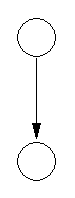
\includegraphics{figures/dp1_pspdftex.eps}}
\end{minipage}
&
\begin{lstlisting}[mathescape=true,language=C]
int main() {
 bool x;
 unsigned char y;
 x=1;
 y=(x+1)&0x3;
}
\end{lstlisting}
\\
\hline
\end{tabular}
\caption{Dependencies between combinational elements}
\label{dp1}
\end{figure}

%
%\textbf{A latch fed by the output of a combinational gate}
\begin{figure}
\scriptsize  
\begin{tabular}{l|l|l}
\hline
  Verilog & Dataflow Graph & Software netlist \\
\hline
\begin{lstlisting}[mathescape=true,language=Verilog]
module M(in1, in2, 
      out1, out2);
input in1, in2;
output reg out1,
output reg out2;
wire t1;
assign t1=out1;
always @(in1) begin
out1 <= in1;
end
always@(t1) begin
out2 <= t1;
end
endmodule
\end{lstlisting}
&
\begin{minipage}{1.8cm}
\centering
\scalebox{.5}{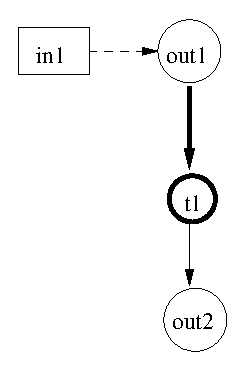
\includegraphics{figures/dp2_pspdftex.eps}}
\end{minipage}
&
\begin{lstlisting}[mathescape=true,language=C]
int M(
bool in1,bool in2, 
bool *out1,
bool *out2) 
{
 bool t1;
 *out1=in1;
 t1=*out1;
 *out2=t1;
}
\end{lstlisting}
\\
\hline
\end{tabular}
\caption{Dependencies between latches and combinational logic}
\label{dp2}
\end{figure}


%\textbf{A latch fed by the output of another latch}
%
\begin{figure}
\scriptsize
\begin{tabular}{l|l|l}
\hline
  Verilog & Dataflow Graph & Software netlist \\
\hline
\begin{lstlisting}[mathescape=true,language=Verilog]
module M(in1, in2, 
      out1, out2);
input in1, in2;
output reg out1, out2;

always @(in1) begin
out1 <= in1;
end

always@(out1) begin
out2 <= out1;
end
endmodule
\end{lstlisting}
&
\begin{minipage}{2.0cm}
\centering
\scalebox{.5}{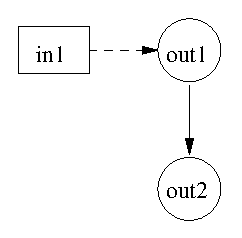
\includegraphics{figures/dp3_pspdftex.eps}}
\end{minipage}
&
\begin{lstlisting}[mathescape=true,language=C]
int M(
bool in1,bool in2, 
bool *out1,*out2) {
 *out1=in1;
 *out2=*out1;
}
\end{lstlisting}
\\
\hline
\end{tabular}
\caption{Dependencies between latches}
\label{dp3}
\end{figure}
%
\Omit{
\textbf{A latch fed by combinational inputs}
%
\begin{figure}[t]
\scriptsize
\begin{tabular}{l|l|l}
\hline
  Verilog & Dataflow Graph & Software netlist \\
\hline
\begin{lstlisting}[mathescape=true,language=Verilog]
module M(in1, in2, out1, out2);
input in1, in2;
output reg out1, out2;

always @(in1) begin
out1 <= in1;
end

always@(in2) begin
out2 <= in2;
end
endmodule
\end{lstlisting}
&
\begin{minipage}{3.0cm}
\centering
\scalebox{.5}{\import{chapter3/figures/}{dp1.pspdftex}}
\end{minipage}
&
\begin{lstlisting}[mathescape=true,language=C]
int M(bool in1, bool in2, 
      bool *out1, *out2) {
 *out1=in1;
 *out2=in2;
}
\end{lstlisting}
\\
\hline
\end{tabular}
\caption{Dependencies between latch and combinational inputs}
\label{dp4}
\end{figure}
}
%
\Omit{For designs with inter-modular combinational paths or combinational loops,
the combinational signals (wire variables) may settle after several
executions before the next clock cycle.  The combinational exchanges between
modules depends on the stability condition for the combinational signals and
thus it is necessary to execute the combinational logic until the stability
condition is reached.  Determining such stability condition for large
circuits is hard.  An alternative way to handle combinational exchanges
between modules is by using assumptions over the signals that encode
combinational logic in the respective modules following synthesis semantics. 
An example using the latter approach is given at
\url{http://www.cprover.org/hardware/v2c/}.
}
%
\subsubsection{Inter-Modular Dependency Analysis}
%
Modules in Verilog communicate with each other through their input or output
ports. Most practical designs are modular in nature, where the top-level 
module delegates specific tasks to the sub-modules.
%through the input ports of sub-module and receive output from 
%the sub-module upon completion of the task.  
Modules and sub-modules executes \emph{in-tandem}, that is, a
module is \emph{not} blocked when it invokes a sub-module. 


An example of inter-modular communication can be illustrated
using the design in figure~\ref{figure:equivalence}.  The top-level 
module \texttt{main} invokes the submodule \texttt{M}.  
The equivalent translation in C (shown in right of figure~\ref{figure:equivalence}) 
preserves the modular structure. 
%
Another example of inter-modular communication is a \emph{combinational feedback loop} 
where participating modules exchange combinational data until a stability condition is reached.  
%
Determining this kind of stability condition completely automatically 
is difficult for large circuits.  Hence, manual translation is performed in such cases.
%  
\subsection{Limitations of V2C Translator}~\label{v2clim}
%  
V2C does not support automatic translation of RTL designs that contain 
the following design features -- a) Multi-clock designs~\cite{multiclock}, 
b) Transparent latches~\cite{DBLP:conf/glvlsi/ChandraWA98}, 
c) Combinational feedback loop, and d) Circular module dependency. 
%  
%
In this paper, we present an automatic translation and verification 
of the RTL designs that do not contain the above design features.   
%  
We now briefly demonstrate the complexity of manually translating 
a design that contains combinational feedback loop.  
Figure~\ref{figure:comb-loop} gives a Verilog design with 
combinational feedback loop on the left.  The right side of 
Figure~\ref{figure:comb-loop} gives the equivalent software netlist, 
which is translated manually. 
%  
The Verilog module {\em foo} is partitioned into two separate modules during
translation -- a combinational module, {\em foo\_comb} and a sequential module,
{\em foo\_seq}.  The combinational exchanges between the Verilog modules {\em top}
and {\em foo} continues until the values of a and z becomes stable, which in 
this case is equal to the width of these registers (32-bit).  This stability 
condition is manually identified and modeled in the software netlist design 
by invoking the procedure {\em foo\_comb} from the {\em main} routine
32 times, followed by a call to the sequential module {\em foo\_seq} which simply
updates the register $y$.  
%  
Note that the assertion given by $(y==loopback)$ in Figure~\ref{figure:comb-loop} 
holds true in the RTL as well as the software netlist design, which is established 
using off-the-shelf hardware and software model checkers respectively.   
%
\begin{figure}[htbp]
\scriptsize
\begin{tabular}{l|l}
\hline
Verilog & Software netlist \\
\hline
\begin{lstlisting}[mathescape=true,language=Verilog]
module M(c,a,z,y);
input c;
input [31:0] a;
output [31:0] z;
output reg [31:0] y;
assign z[0]=c;
assign z[31:1]=a[30:0];
always @(posedge clk)
y<=z;
endmodule

module top();
wire [31:0] loopback;
wire [31:0] y;
foo f(.c(1),.a(loopback),
      .z(loopback),.y());
assert property 
       (y==loopback); 
endmodule 
\end{lstlisting}
&
\begin{lstlisting}[mathescape=true,language=C]
struct state_elements_M {
  unsigned int y;
};
struct state_elements_M sM;

void foo_comb(bool c, unsigned int a,
unsigned int *z, unsigned int *y) {
  *z=(*z&0xfffffffe) | (c & 0x1);
  *z=(*z&0x00000001) | 
     ((a&0x7fffffff)<<1); }
void foo_seq(bool c, unsigned int a,
unsigned int *z, unsigned int *y) {
 sM.y = *z;
}
void top() {
 unsigned int y, loopback;
 for(i=1;i<33;i++)
  foo_comb(1,loopback,&loopback,&y);
  foo_seq(1,loopback,&loopback,&y);
  assert(y==loopback); 
}
\end{lstlisting}
\\
\hline
\end{tabular}
\caption{Manual translation of combinational feedback loop}
\label{figure:comb-loop}
\end{figure}
%
